\section{BGP routing table}
\label{sec:bgp}

In this section we present an evaluation of the global routing table from 2003
to 2009. We first analyze contributing causes to the growth of the global
routing table. This involves assessing a measure of how well ISPs tend to use
an allocated address space and how allocated address blocks are subdivided. The
second point of interest is to analyze the contents of the BGP routing table
itself. This includes determining the extent that IP prefix announcements
overlap (i.e., how many individual prefixes are also parts of bigger prefixes
present in the same routing table). We also discuss a measure of the stability
of the routing table contents. For this measurement, we calculate the time
period during which an individual prefix was visible to the BGP monitor.
Finally, in an analogous fashion to the previous section, we present an
analysis of the BGP routing table dynamics grouped by the geographical region.
We conclude with identifying countries with the largest number of announced
prefixes.

%%%%%%%%%%%%%%%%%%%%%%%%%%%%%%%%%%%%%%%%%%%%%%%%%%%%%%%%%%%%%%%%%%%%%%%%%%%%%
%%%%%%%%%%%%%%%%%%%%%%%%%%%%%%%%%%%%%%%%%%%%%%%%%%%%%%%%%%%%%%%%%%%%%%%%%%%%%
%%%%%%%%%%%%%%%%%%%%%%%%%%%%%%%%%%%%%%%%%%%%%%%%%%%%%%%%%%%%%%%%%%%%%%%%%%%%%
\subsection{Analysis of BGP table growth factors}
%%%%%%%%%%%%%%%%%%%%%%%%%%%%%%%%%%%%%%%%%%%%%%%%%%%%%%%%%%%%%%%%%%%%%%%%%%%%%
%%%%%%%%%%%%%%%%%%%%%%%%%%%%%%%%%%%%%%%%%%%%%%%%%%%%%%%%%%%%%%%%%%%%%%%%%%%%%
%%%%%%%%%%%%%%%%%%%%%%%%%%%%%%%%%%%%%%%%%%%%%%%%%%%%%%%%%%%%%%%%%%%%%%%%%%%%%

The BGP routing table is growing at a rate significantly higher than the pace
that RIRs are allocating IP blocks. Across all BGP monitors we observed, the
average number of entries in the global routing table is more than 3 times the
number of IP blocks that RIRs have allocated (refer Figure~\ref{fig:BGP vs
RIR}). This multiplication in size reflects two primary practices. First, ISPs
tend to subdivide allocated IP blocks into several individual prefixes and
announce them separately. Such behavior is typical, for example, among
transnational providers as well as among ISP customers that have been lent
parts of their service providers' address space and in turn independently
announce subdivided IP address blocks. Second, various traffic engineering
techniques (traffic balancing, multihoming, etc.) give rise to situations where
the same address block is covered by several announced prefixes.

\subsubsection{IP block fragmentation}

The contents of the BGP routing table consist of IP prefixes that either match,
fragment, or aggregate various IP allocation blocks.
Figure~\ref{fig:fragmentation} shows the correlation between allocated IP
blocks and announced IP prefixes and the relative proportions of these three
categories over time. The \emph{matched} curve in the figure represents IP
blocks that are announced in the routing table in the exact form as they were
issued by RIRs. An example of a matched prefix announcement is an appearance in
the table of a /22 prefix (equivalent to 1,024 IP addresses) that was issued in
just that form by an ISP. As is evident in the figure, the number of matched
prefixes accounts for 1/6 the total number of BGP entries at the present time,
with the trend that this fraction is growing smaller over time.

\begin{figure}[htbp]
	\centering
		\includegraphics[width=\columnwidth]{05_matched_fragmented/frag-3}
	\caption{Dynamics of matched, fragmented, and aggregated IP prefixes in BGP announcements}
	\label{fig:fragmentation}
\end{figure}

ISPs are evidently not inclined to distribute address space often in the form
in which it was allocated. For various possible reasons (e.g., geographical
dispersion), ISPs split up allocated blocks into a number of sub-blocks and
announce each of these independently. The \emph{fragmented} curve in
Figure~\ref{fig:fragmentation} represents these subdivided blocks, which
account for more than 83\% of all entries in the global routing table. IP block
fragmentation poses one of the primary concerns for future scalability of the
BGP routing table.

The lowest curve, \emph{aggregated}, represents IP prefix announcements that
cover several allocated IP blocks. For these cases---in contrast to
fragmentation---ISPs that have several adjacent IP block allocations simply
announce them as a single IP prefix. As the figure illustrates, this
aggregation technique is rarely employed to any measure. Its primary intent, to
reduce the number of entries in the routing table, is outweighed for more often
by other policy routing choices. The number of aggregated prefixes in 2003 was
1,400. By 2009 this number increased only marginally, to just under 2,000
prefixes, accounting for under 1\% of the entire routing table and reasonably
considered negligible in impact.

This observed behavior has a measure of relevance to future IPv6 deployment.
ISPs tend not to announce their allocated IP spaces in their original form.
Significantly, this behavior occurs regardless of the size of IP block that an
ISP was allocated. With regard to IPv6 deployment, the significance of this
point is as follows. According to current RIR policy, the minimum allocation
for an IPv6 block is /32 \cite{APNIC:2009:IPv6-Address}. In terms of expense,
the price of an IPv6 /32 block is the same as for a /19 or /20 IPv4 address
block \cite{ARIN:2009:Annual-Fee-Scedule}, meaning for an equivalent cost of
obtaining under 10,000 IPv4 prefixes, ISPs can be assigned an IPv6 block of a
size several orders of magnitude larger than the entire IPv4 space at present.
If allocations of large blocks continue, it is likely to mitigate the problem
of multiple, non-adjacent IP block allocations per customer. However, without a
major change in the BGP protocol aimed at lessening incentives to announce
fragmented IP prefixes, increasing the size of the IP block will not
significantly assist in reducing the size of global routing table. Table size
reduction stems only from aggregatable and matching IP prefixes. In other
words, only ISPs that currently use all allocated IP space as a single IP block
(i.e., matched or aggregated) would have any likelihood of using a bigger space
provided in IPv6 also as a single block. We conclude that the upper bound of IP
space announcement optimization is limited by the number of matched prefixes,
which currently stands at less than 17\% of all prefixes.

\subsubsection{Duplicate announcements of IP blocks}

The BGP routing table has a consistent pattern of containing a large number of
prefix ranges that duplicate each other (Figure~\ref{fig:covered}). IP address
coverage duplication assists calculating an actual route by matching the
destination address with the longest available prefix.  Address duplication in
a routing table is, in theory, an effective way to reduce the size of the
routing table itself. The following example illustrates this point: If we
consider an ISP that owns a /8 address block and that wants a particular /24
block routed in a special way, using a different path than the rest of the
block, it is much more effective to use a small duplication of address space
and only two entries in the routing table (the /8 and the /24 prefixes) than
avoiding duplication and announcing 65,536 individual /24 prefixes.

\begin{figure}[htbp]
	\centering
		\includegraphics[width=\columnwidth]{06_covered/cover-3}
	\caption{Relative numbers of \emph{covered}, \emph{covering}, and \emph{unique} IP prefixes among BGP announcements}
	\label{fig:covered}
\end{figure}

Our observations indicate that ISPs extensively use the fundamental IP routing
feature of longest-prefix matching. As Figure~\ref{fig:covered} shows by the
\emph{1-level} and \emph{unique} curves, the number of IP prefixes in BGP table
which are covered by exactly one bigger prefix is nearly the same as the number
of unique prefixes (i.e., base prefixes). There is moreover a substantial
number of prefixes that have several layers of coverage (several duplication
levels---refer to \emph{2+-level} curve).

These high proportions of 1-level and 2+-level covered prefixes indicate there
are other incentives and benefits for prefix duplication, in addition to the
theoretical routing table optimization. One factor we consider is a
multi-provider connection for end-networks (so-called multihoming of \emph{stub
networks}). According to Oliveira et al.
\cite{Oliveira:2007:Observing-the-evolution}, more than 70\% of all
announcements belong to multihomed stub networks. In other words, the global
routing table was adopted to serve local or semi-local routing interests for
most customers. Since these routing interests extend out on a primarily local
scale, it would seem unlikely that the outside world would follow widely
divergent routing paths to reach various providers' connections to a multihomed
customer (a stub network). Thus while the need for covered prefixes is evident
to accommodate these routing preferences, they need not be shared universally
in routing tables. We conclude that to significantly reduce the size of the BGP
routing table, there should be counter-incentives to IP prefix fragmentation.
As an area of further research, for example, separate means for multihoming and
traffic engineering tasks might be provided.

%%%%%%%%%%%%%%%%%%%%%%%%%%%%%%%%%%%%%%%%%%%%%%%%%%%%%%%%%%%%%%%%%%%%%%%%%%%%%
%%%%%%%%%%%%%%%%%%%%%%%%%%%%%%%%%%%%%%%%%%%%%%%%%%%%%%%%%%%%%%%%%%%%%%%%%%%%%
%%%%%%%%%%%%%%%%%%%%%%%%%%%%%%%%%%%%%%%%%%%%%%%%%%%%%%%%%%%%%%%%%%%%%%%%%%%%%
\subsection{Analysis of the BGP table contents}
%%%%%%%%%%%%%%%%%%%%%%%%%%%%%%%%%%%%%%%%%%%%%%%%%%%%%%%%%%%%%%%%%%%%%%%%%%%%%
%%%%%%%%%%%%%%%%%%%%%%%%%%%%%%%%%%%%%%%%%%%%%%%%%%%%%%%%%%%%%%%%%%%%%%%%%%%%%
%%%%%%%%%%%%%%%%%%%%%%%%%%%%%%%%%%%%%%%%%%%%%%%%%%%%%%%%%%%%%%%%%%%%%%%%%%%%%

In this part we examine the contents that comprise the BGP routing table. By
analyzing changes in its contents over the period from 2003 to 2009 we can
deduce current trends and demands for the IP space. Later in this part, we
share the distribution of prefix sizes announced in the table, the lifespan
(longevity) of IP prefix announcements, and the distribution of the IP space
from a geographical standpoint.

\subsubsection{Lengths of announced IP prefixes}

Critical questions in the global routing system are the following: (1) What is
an optimal length of IP prefix to allocate to customers? and (2) What is the
optimal algorithm to select a right prefix to allocate (in other words, how
much space should RIRs or ISPs reserve after an allocated block to accommodate
repeated requests from the same customer, and still maintain the customer's
allocations adjacent to each another, reducing fragmentation)? A number of
solutions propose to resolve the latter question, including sequential and
bisection allocation schemes and the GAP algorithm
\cite{Wang:2007:Reduce-IP-Address}. The former is still an open research
question.

To explore an answer to the first question, we present current statistics of
prefix lengths that have appeared in the routing table since 2003.
 Figure~\ref{fig:bgp prefix distribution} presents the distribution of
announced prefix lengths, classified by each year. The majority of the global
routing table entries are /24-length prefixes and account for more than 53\% of
entries. Among statistics for /24 prefixes, it is notable that the number of
/24 prefixes has nearly doubled between 2003 and 2009. At the same time, the
number of allocated blocks actually /24 in size is 4 times smaller (refer
Figure~\ref{fig:IP allocations}). This again gives evidence that a large number
of stub networks (i.e., relatively small customer networks) use announcements
of small address blocks to implement multi-provider connectivity.

\begin{figure}[htbp]
	\centering
		\includegraphics[width=\columnwidth]{02_prefixes/01_bgp_prefixes_zoom}
	\caption{Distribution of announced IP prefix lengths}
	\label{fig:bgp prefix distribution}
\end{figure}

Several other observations can be made from Figure~\ref{fig:bgp prefix
distribution}. Prefix lengths of /16--/23 (in comparison to /24 lengths) have
relatively the same level of popularity in the global routing table, among
which /17 and /18 constitute the least popular. The most dynamic prefixes among
this group over the 6 years are /20 and /21 (2.8 and 3.7 times growth,
respectively), and the least dynamic is /16 (1.4 times growth). Another
interesting observation concerns /16 prefixes. From among the most numerous
kinds of prefix lengths announced in the routing table (/16--/24), only the
number of /16 prefixes announced in the routing table closely matches the
number of allocations (again refer Figure~\ref{fig:IP allocations}). All the
other most popular prefix lengths comprising the routing table have markedly
higher counts of announced prefixes in the table than were originally
allocated, giving further indication of prevalent fragmentation.

The rest of the prefixes (shorter than /16, longer than /24) have a marginal
presence in the global routing table.  Together, they number less than 8,000
prefixes ($<$3\%). This fact testifies to a small number of entities having large
(/8--/15) prefixes, and a small number of a tiny customer networks (prefixes
/25--/32) with a multi-provider connectivity.

The results in this section are additional evidence of the tight relationship
between global routing table growth and IP space fragmentation and duplication.
If we could suppress the majority of non-global related (i.e., locally
concerned) announcements, such as bursts of /24 prefixes due to local traffic
engineering, local and semi-local multihoming support, etc., the size of the
global routing table would be significantly reduced.

\subsubsection{Longevity distribution of BGP entries}

Another aspect of the BGP announcement analysis is determining the stability of
the global routing table. The distribution of prefix longevity is shown in
Figure~\ref{fig:bgp ages}. The bar on the far right of the graph indicates that
more than 15\% of the global routing table never changes over the course of our
period of study. On the other, far-left side, approximately another 15\% of the
prefixes
% (if we compare to the global routing table size in 2009)
 are active for only a short period of time. A small part of these
short-lived prefixes is likely comprised of spammers, who are known to hijack
someone's (or nobody's) prefix, announce it for a brief time, and send
virtually untraceable spam messages
\cite{Ramachandran:2006:Understanding-the-network-level}. Another portion of
short-lived prefixes can be attributed to configuration errors. The rest can be
explained by normal BGP operations, where some prefix becomes visible briefly
in such circumstances as when a primary network channel malfunctions.

\begin{figure}[htbp]
	\centering
		\includegraphics[width=\columnwidth]{08_ages/ages-4}
	\caption{Longevity of prefixes in BGP announcements}
	\label{fig:bgp ages}
\end{figure}

Excluding the unchanging portion of the BGP table contents shown in
Figure~\ref{fig:bgp ages}, the prefix longevity distribution follows to some
extent the exponential distribution function. In other words, announced
prefixes are likely to have a small longevity.  Besides a fixed number of
highly stable routes (15\%), the tapering-off shape of the distribution
suggests it is unlikely that a given route is visible for very long time. This
observation underscores that the composition of the routing table is highly
dynamic.

\subsubsection{BGP announcements by geographical region}

Finally, in examining the global routing table content, we present a
country-based analysis of the distribution of globally announced IP prefixes.
As with the allocation data, fixed-time snapshots point out the major
contributors to the global routing table and give an understanding of the
Internet's penetration throughout the world.

Table~\ref{tab:top25 bgp prefixes 2003} lists the top 25 contributors to the
global routing table in 2003 and gives the corresponding actual IP address
space that the announced prefixes cover. Table~\ref{tab:top25 bgp ip space
2003} gives an alternative representation for the BGP data snapshot from 2003,
where countries are listed in descending order by the number of IP addresses
covered by BGP announcements. To achieve these results, we matched announced
address spaces with corresponding allocated address spaces.  Due to the limited
nature of our IP prefix country association technique, there is a considerable
portion of the prefixes for which it was not possible to establish such an
association. Globally announced prefixes with undetermined ownership (shown as
\emph{Unknown}) in fact constitute the second largest contributor to the
routing table in 2003, after the United States. Holding third and fourth place
in 2003 were Australia and Canada. It should be mentioned that geographical
distributions, both of announced IP prefixes (Figure~\ref{fig:prefix distr})
and of announced IP space (Figure~\ref{fig:size distr}), have a stable,
quasi-exponential tapering shape.  The plot lines in both cases show minimal
variation in shape of the plot between 2003 and 2009.

\begin{figure}[htbp]
	\centering
		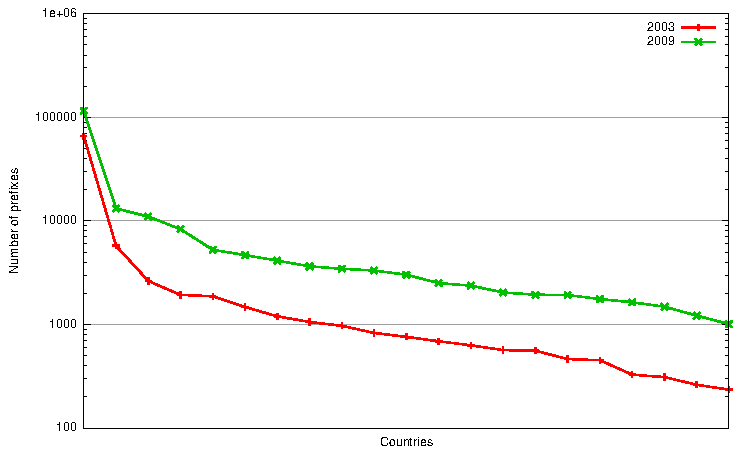
\includegraphics[width=\columnwidth]{01_bgp_ip_size/prefix-distr}
	\caption{Geographical distribution of globally announced IP prefixes (log scale)}
	\label{fig:prefix distr}
\end{figure}

\begin{figure}[htbp]
	\centering
		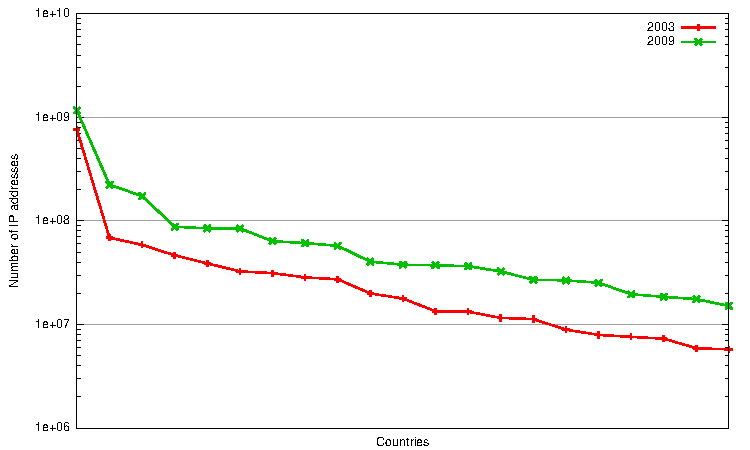
\includegraphics[width=\columnwidth]{01_bgp_ip_size/size-distr}
	\caption{Geographical distribution of globally announced IP space (log scale)}
	\label{fig:size distr}
\end{figure}

Tables~\ref{tab:top25 bgp prefixes 2009} and ~\ref{tab:top25 bgp ip space 2009}
present estimates for 2009 of the top 25 contributors to the global routing
table and the top 25 countries with the most announced address space. Again,
matched side-by-side with their 2003 counterparts, they provide easy comparison
of changes over time.  All countries contribute in greater numbers to the BGP
table. At the same time, the number of prefixes with undetermined ownership
(and the corresponding IP space) diminishes substantially by about half. The
United States retains its leading position. Meanwhile the ordering of the rest
contributors has significantly changed. South Korea has become the second major
contributor to the size of the global routing table, and China, Australia, and
India (having roughly the same number of announcements) rank third.

In terms of IP space usage, China, Japan, the European Union, Germany, and
South Korea are responsible over the most amount of announced address space
behind the United States. These four countries are a different ordering from
the number of announcements attributed in the routing table to a given country
(Table~\ref{tab:top25 bgp prefixes 2009}). This fact highlights that some
countries announce a large number of relatively small prefixes (e.g., in South
Korea one prefix on average covers 5,900 addresses), and some announce a small
number of large prefixes (e.g., in Japan one prefix covers on average 37,200
addresses). If this difference in usage efficiency occurs because of additional
government regulations, then for future IPv6 deployment, a similar host of
regulations should be considered globally.

 % are extremely efficient from BGP point of view

An alternative way to represent each country's contribution to the global
routing table is through color-coded diagrams in Figures~\ref{fig:bgp prefixes
2003}--\ref{fig:bgp ip space asia 2009}.%
%
\footnote{%
An extended number of interactive colored maps for years 2003--2009 are
available at \url{http://maps.iu4.ru}}%
%
~The figure pairs~\ref{fig:bgp prefixes 2003} \&~\ref{fig:bgp prefixes 2009},
as well as~\ref{fig:bgp ip space 2003} \&~\ref{fig:bgp ip space 2009}, make it
possible to trace the regional Internet growth dynamics. Figures~\ref{fig:bgp
prefixes asia 2009} and~\ref{fig:bgp ip space asia 2009} emphasize once again
differences of the varying effectiveness of IP space utilization (e.g., Japan
has many more addresses per announced prefix than compared to India or South
Korea).


\begin{table*}[tp]
%%%%%%%%%%%%%%%%%%%%%%%%%%%%%%%%%%%%%%%%%%%%%%%%%%%%%%%%%%%%%%%%%%%%%%%%%%%%%%%%
%% TOP announced prefixes
%%%%%%%%%%%%%%%%%%%%%%%%%%%%%%%%%%%%%%%%%%%%%%%%%%%%%%%%%%%%%%%%%%%%%%%%%%%%%%%%
\begin{minipage}[t]{0.48\textwidth}
% \begin{table}[p]
	\begin{center}
	\caption{Top 25 countries with the most number of announced prefixes in BGP table on \textbf{January 1, 2003}}
	\label{tab:top25 bgp prefixes 2003}
	\begin{tabular}{|l||l|r|r|} %\hline
		\hline
		&      \bf Country		&    Prefixes   &       IP space 		\tabularnewline \hline 
1       &       US      		&       65849   &       759,792,816     \tabularnewline %\hline
2       &       \emph{Unknown}	&       6258    &       68,926,314      \tabularnewline %\hline
3       &       Australia       &       5762    &       17,822,159      \tabularnewline %\hline
4       &       Canada  		&       5612    &       38,912,924      \tabularnewline %\hline
5       &       Japan   		&       2633    &       58,905,280      \tabularnewline %\hline
6       &       South Korea     &       2441    &       27,334,687      \tabularnewline %\hline
7       &       Germany			&       1934    &       46,556,556      \tabularnewline %\hline
8       &       India  			&       1931    &       2,943,040       \tabularnewline %\hline
9       &       UK     			&       1873    &       32,626,649      \tabularnewline %\hline
10      &       China  			&       1615    &       28,522,130      \tabularnewline %\hline
11      &       Argentina       &       1477    &       2,017,448       \tabularnewline %\hline
12      &       Hong Kong       &       1261    &       5,621,473       \tabularnewline %\hline
13      &       Sweden  		&       1198    &       11,280,533      \tabularnewline %\hline
14      &       France  		&       1148    &       31,320,040      \tabularnewline %\hline
15      &       Mexico  		&       1059    &       5,275,520       \tabularnewline %\hline
16      &       Romania 		&       994     &       667,136 		\tabularnewline %\hline
17      &       Russia  		&       972     &       5,911,712       \tabularnewline %\hline
18      &       Chile   		&       834     &       2,098,161       \tabularnewline %\hline
19      &       Indonesia       &       830     &       1,170,560       \tabularnewline %\hline
20      &       Italy   		&       791     &       13,324,288      \tabularnewline %\hline
21      &       Brazil  		&       760     &       11,580,416      \tabularnewline %\hline
22      &       Taiwan  		&       708     &       13,448,168      \tabularnewline %\hline
23      &       Netherlands     &       689     &       19,939,341      \tabularnewline %\hline
24      &       European Union  &       687     &       2,707,383       \tabularnewline %\hline
25      &       Finland 		&       630     &       7,307,018       \tabularnewline %\hline
% 26      &       South Africa    &       618     &       5,762,180       \tabularnewline %\hline
% 27      &       New Zealand     &       566     &       3,828,620       \tabularnewline %\hline
% 28      &       Switzerland     &       560     &       7,937,424       \tabularnewline %\hline
% 29      &       Thailand        &       559     &       1,877,060       \tabularnewline %\hline
% 30      &       Spain   		&       511     &       8,921,568       \tabularnewline %\hline
	\hline
	\end{tabular}
	\end{center}
% \end{table}
\end{minipage}
%
\quad
%
\begin{minipage}[t]{0.48\textwidth}
% \begin{table}[p]
	\begin{center}
	\caption{Top 25 countries with the most number of announced prefixes in BGP table on \textbf{April 23, 2009}}
	\label{tab:top25 bgp prefixes 2009}
	\begin{tabular}{|l||l|r|r|r|}
		\hline
		&      \bf Country		& \bf Prefixes  &       \bf IP space 	& \bf Change$^{*}$ 	\tabularnewline \hline 
1       &       US      		&       115780  &       1,170,481,177   & 1.54			\tabularnewline %\hline
2       &       South Korea     &       14308   &       84,553,300      & 3.09			\tabularnewline %\hline
3       &       China  			&       13188   &       223,990,021     & 7.85			\tabularnewline %\hline
4       &       Australia       &       11329   &       37,818,072      & 2.12			\tabularnewline %\hline
5       &       India   		&       11022   &       17,575,040      & 5.97			\tabularnewline %\hline
6       &       Russia  		&       8650    &       26,664,224      & 4.51			\tabularnewline %\hline
7       &       Canada  		&       8328    &       57,471,348      & 1.48			\tabularnewline %\hline
8       &       Romania 		&       5729    &       7,348,881       & 11.02			\tabularnewline %\hline
9       &       UK      		&       5269    &       63,871,082      & 1.96			\tabularnewline %\hline
10      &       European Union  &       4937    &       87,825,582      & 32.44			\tabularnewline %\hline
11      &       Japan   		&       4674    &       173,789,965     & 2.95			\tabularnewline %\hline
12      &       Brazil  		&       4643    &       40,429,504      & 3.49			\tabularnewline %\hline
13      &       Argentina       &       4142    &       9,721,411       & 4.82			\tabularnewline %\hline
14      &       Germany 		&       4035    &       84,904,642      & 1.82			\tabularnewline %\hline
15      &       Mexico  		&       3648    &       19,583,832      & 3.71			\tabularnewline %\hline
16      &       Indonesia       &       3562    &       5,248,256       & 4.48			\tabularnewline %\hline
17      &       Hong Kong       &       3459    &       14,764,300      & 2.63			\tabularnewline %\hline
18      &       \emph{Unknown}	&       3393    &       37,265,411      & 				\tabularnewline %\hline
19      &       Bulgaria        &       3325    &       4,439,040       & 7.72			\tabularnewline %\hline
20      &       Colombia        &       3029    &       4,901,340       & 11.86			\tabularnewline %\hline
21      &       Ukraine 		&       3028    &       5,547,136       & 7.67			\tabularnewline %\hline
22      &       Egypt  			&       2992    &       3,854,848       & 4.60			\tabularnewline %\hline
23      &       France 			&       2511    &       61,070,996      & 1.95			\tabularnewline %\hline
24      &       Taiwan 			&       2511    &       36,623,744      & 2.72			\tabularnewline %\hline
25      &       Chile  			&       2375    &       6,101,376       & 2.91			\tabularnewline %\hline
% 26      &       Poland 			&       2341    &       15,122,881      & 4.06			\tabularnewline %\hline
% 27      &       Thailand        &       2039    &       7,210,800       & 3.84			\tabularnewline %\hline
% 28      &       Spain   		&       1989    &       25,315,136      & 2.84			\tabularnewline %\hline
% 29      &       Sweden  		&       1942    &       18,532,345      & 1.64			\tabularnewline %\hline
% 30      &       Turkey  		&       1940    &       14,309,632      & 6.41			\tabularnewline %\hline
	\hline
	\end{tabular}
	\end{center}
	
	\small	$^{*}$ -- Relative change in number of prefixes in BGP announcements from January 1, 2003 and April 23, 2009
% \end{table}
\end{minipage}

\vspace{1cm}

%%%%%%%%%%%%%%%%%%%%%%%%%%%%%%%%%%%%%%%%%%%%%%%%%%%%%%%%%%%%%%%%%%%%%%%%%%%%%%%%
%% TOP announced IP space
%%%%%%%%%%%%%%%%%%%%%%%%%%%%%%%%%%%%%%%%%%%%%%%%%%%%%%%%%%%%%%%%%%%%%%%%%%%%%%%%
\begin{minipage}[t]{0.48\textwidth}
% \begin{table}[p]
	\begin{center}
	\caption{Top 25 countries with the most number of announced IP space in BGP table on \textbf{January 1, 2003}}
	\label{tab:top25 bgp ip space 2003}
	\begin{tabular}{|l||l|r|r|}
		\hline
		&      \bf Country		&    Prefixes   &       IP space 		\tabularnewline \hline 
1       &       US      		&       65849   &       759,792,816     \tabularnewline %\hline
2       &       \emph{Unknown} 	&       6258    &       68,926,314      \tabularnewline %\hline
3       &       Japan   		&       2633    &       58,905,280      \tabularnewline %\hline
4       &       Germany 		&       1934    &       46,556,556      \tabularnewline %\hline
5       &       Canada  		&       5612    &       38,912,924      \tabularnewline %\hline
6       &       UK      		&       1873    &       32,626,649      \tabularnewline %\hline
7       &       France  		&       1148    &       31,320,040      \tabularnewline %\hline
8       &       China   		&       1615    &       28,522,130      \tabularnewline %\hline
9       &       South Korea     &       2441    &       27,334,687      \tabularnewline %\hline
10      &       Netherlands     &       689     &       19,939,341      \tabularnewline %\hline
11      &       Australia       &       5762    &       17,822,159      \tabularnewline %\hline
12      &       Taiwan  		&       708     &       13,448,168      \tabularnewline %\hline
13      &       Italy   		&       791     &       13,324,288      \tabularnewline %\hline
14      &       Brazil  		&       760     &       11,580,416      \tabularnewline %\hline
15      &       Sweden  		&       1198    &       11,280,533      \tabularnewline %\hline
16      &       Spain   		&       511     &       8,921,568       \tabularnewline %\hline
17      &       Switzerland     &       560     &       7,937,424       \tabularnewline %\hline
18      &       Norway  		&       262     &       7,591,936       \tabularnewline %\hline
19      &       Finland 		&       630     &       7,307,018       \tabularnewline %\hline
20      &       Russia  		&       972     &       5,911,712       \tabularnewline %\hline
21      &       South Africa    &       618     &       5,762,180       \tabularnewline %\hline
22      &       Hong Kong       &       1261    &       5,621,473       \tabularnewline %\hline
23      &       Austria 		&       317     &       5,405,664       \tabularnewline %\hline
24      &       Mexico  		&       1059    &       5,275,520       \tabularnewline %\hline
25      &       Denmark 		&       196     &       4,169,984       \tabularnewline %\hline
% 26      &       New Zealand     &       566     &       3,828,620       \tabularnewline %\hline
% 27      &       Belgium 		&       175     &       3,796,224       \tabularnewline %\hline
% 28      &       Poland  		&       273     &       3,721,216       \tabularnewline %\hline
% 29      &       Malaysia        &       235     &       3,182,400       \tabularnewline %\hline
% 30      &       India   		&       1931    &       2,943,040       \tabularnewline %\hline
	\hline
	\end{tabular}
	\end{center}
	\ \newline\ \newline
% \end{table}
\end{minipage}
%
\quad
%
\begin{minipage}[t]{0.48\textwidth}
% \begin{table}[p]
	\begin{center}
	\caption{Top 25 countries with the most number of announced IP space in BGP table on \textbf{April 23, 2009}}
	\label{tab:top25 bgp ip space 2009}
	\begin{tabular}{|l||l|r|r|r|}
		\hline
		&      \bf Country		& \bf Prefixes  &       \bf IP space 	& \bf Change$^{*}$ 	\tabularnewline \hline 
1       &       US      		&       115780  &       1,170,481,177   & 1.76			\tabularnewline %\hline
2       &       China   		&       13188   &       223,990,021     & 8.17			\tabularnewline %\hline
3       &       Japan   		&       4674    &       173,789,965     & 1.78			\tabularnewline %\hline
4       &       European Union  &       4937    &       87,825,582      & 7.19			\tabularnewline %\hline
5       &       Germany 		&       4035    &       84,904,642      & 2.09			\tabularnewline %\hline
6       &       South Korea     &       14308   &       84,553,300      & 5.86			\tabularnewline %\hline
7       &       UK      		&       5269    &       63,871,082      & 2.81			\tabularnewline %\hline
8       &       France  		&       2511    &       61,070,996      & 2.19			\tabularnewline %\hline
9       &       Canada  		&       8328    &       57,471,348      & 1.48			\tabularnewline %\hline
10      &       Brazil  		&       4643    &       40,429,504      & 6.11			\tabularnewline %\hline
11      &       Australia       &       11329   &       37,818,072      & 1.97			\tabularnewline %\hline
12      &       \emph{Unknown}	&       3393    &       37,265,411      & 				\tabularnewline %\hline
13      &       Taiwan  		&       2511    &       36,623,744      & 3.55			\tabularnewline %\hline
14      &       Italy   		&       1686    &       32,551,268      & 2.13			\tabularnewline %\hline
15      &       Netherlands     &       1883    &       27,122,689      & 2.73			\tabularnewline %\hline
16      &       Russia  		&       8650    &       26,664,224      & 8.90			\tabularnewline %\hline
17      &       Spain   		&       1989    &       25,315,136      & 3.89			\tabularnewline %\hline
18      &       Mexico  		&       3648    &       19,583,832      & 3.44			\tabularnewline %\hline
19      &       Sweden  		&       1942    &       18,532,345      & 1.62			\tabularnewline %\hline
20      &       India   		&       11022   &       17,575,040      & 5.71			\tabularnewline %\hline
21      &       Poland  		&       2341    &       15,122,881      & 8.58			\tabularnewline %\hline
22      &       Hong Kong       &       3459    &       14,764,300      & 2.74			\tabularnewline %\hline
23      &       Turkey  		&       1940    &       14,309,632      & 8.40			\tabularnewline %\hline
24      &       South Africa    &       1218    &       12,969,116      & 1.97			\tabularnewline %\hline
25      &       Argentina       &       4142    &       9,721,411       & 2.80			\tabularnewline %\hline
% 26      &       Vietnam        	&       1010    &       9,514,496       & 50.50			\tabularnewline %\hline
% 27      &       Switzerland     &       1230    &       9,244,448       & 2.20			\tabularnewline %\hline
% 28      &       Denmark 		&       569     &       9,239,192       & 2.90			\tabularnewline %\hline
% 29      &       Malaysia        &       572     &       8,791,684       & 2.43			\tabularnewline %\hline
% 30      &       Finland 		&       469     &       8,691,972       & 0.74			\tabularnewline %\hline
	\hline
	\end{tabular}
	\end{center}
	\small	$^{*}$ -- Relative change in globally announced IP space from January 1, 2003 and April 23, 2009
% \end{table}
\end{minipage}

\end{table*}

% \clearpage

\begin{figure*}[tp]
\centering

%%%%%%%%%%%%%%%%%%%%%%%%%%%%%%%%%%%%%%%%%%%%%%%%%%%%%%%%%%%%%%%%%%
%% BGP counts
%%%%%%%%%%%%%%%%%%%%%%%%%%%%%%%%%%%%%%%%%%%%%%%%%%%%%%%%%%%%%%%%%%
\begin{minipage}[b]{0.48\textwidth}
% \begin{figure}[p]
	\centering
		\includegraphics[trim=0 17px 0px 76px,clip=true,width=\columnwidth]{00_maps/bgp_count_2003}%
		\hspace{-0.98\columnwidth}%
		\includegraphics[width=1cm]{scale_bgp_count}\hspace{-1cm}%
		\hspace{0.98\columnwidth}
	\caption{Geographical distribution of number of announced prefixes on \textbf{January 1, 2003}}
	\label{fig:bgp prefixes 2003}
% \end{figure}
\end{minipage}%
%
\quad
%
\begin{minipage}[b]{0.48\textwidth}
% \begin{figure}[p]
	\centering
		\includegraphics[trim=0 17px 0px 76px,clip=true,width=\columnwidth]{00_maps/bgp_count_2009_2}%
		\hspace{-0.98\columnwidth}%
		\includegraphics[width=1cm]{scale_bgp_count}\hspace{-1cm}%
		\hspace{0.98\columnwidth}
	\caption{Geographical distribution of number of announced prefixes on \textbf{April 23, 2009}}
	\label{fig:bgp prefixes 2009}
% \end{figure}
\end{minipage}

\vspace{0.5cm}

%%%%%%%%%%%%%%%%%%%%%%%%%%%%%%%%%%%%%%%%%%%%%%%%%%%%%%%%%%%%%%%%%%
%% BGP sizes
%%%%%%%%%%%%%%%%%%%%%%%%%%%%%%%%%%%%%%%%%%%%%%%%%%%%%%%%%%%%%%%%%%
\begin{minipage}[b]{0.48\textwidth}
% \begin{figure}[p]
	\centering
		\includegraphics[trim=0 17px 0px 76px,clip=true,width=\columnwidth]{00_maps/bgp_size_2003}%
		\hspace{-0.98\columnwidth}%
		\includegraphics[width=1cm]{scale_bgp_size}\hspace{-1cm}%
		\hspace{0.98\columnwidth}
	\caption{Geographical distribution of announced IP space on \textbf{January 1, 2003}}
	\label{fig:bgp ip space 2003}
% \end{figure}
\end{minipage}%
%
\quad
%
\begin{minipage}[b]{0.48\textwidth}
% \begin{figure}[p]
	\centering
		\includegraphics[trim=0 17px 0px 76px,clip=true,width=\columnwidth]{00_maps/bgp_size_2009_2}%
		\hspace{-0.98\columnwidth}%
		\includegraphics[width=1cm]{scale_bgp_size}\hspace{-1cm}%
		\hspace{0.98\columnwidth}
	\caption{Geographical distribution of announced IP space on \textbf{April 23, 2009}}
	\label{fig:bgp ip space 2009}
% \end{figure}
\end{minipage}

\vspace{0.5cm}

%%%%%%%%%%%%%%%%%%%%%%%%%%%%%%%%%%%%%%%%%%%%%%%%%%%%%%%%%%%%%%%%%%
%% Asia region
%%%%%%%%%%%%%%%%%%%%%%%%%%%%%%%%%%%%%%%%%%%%%%%%%%%%%%%%%%%%%%%%%%
\begin{minipage}[b]{0.48\textwidth}
% \begin{figure}[p]
	\centering
		\includegraphics[trim=0 17px 0px 76px,clip=true,width=\columnwidth]{00_maps/asia_2009_prefixes}%
		\hspace{-0.98\columnwidth}%
		\includegraphics[width=1cm]{scale_bgp_count}\hspace{-1cm}%
		\hspace{0.98\columnwidth}
	\caption{Geographical distribution of number of announced prefixes in Asian region on \textbf{April 23, 2009}}
	\label{fig:bgp prefixes asia 2009}
% \end{figure}
\end{minipage}%
%
\quad
%
\begin{minipage}[b]{0.48\textwidth}
% \begin{figure}[p]
	\centering
		\includegraphics[trim=0 17px 0px 76px,clip=true,width=\columnwidth]{00_maps/asia_2009_space}%
		\hspace{-0.98\columnwidth}%
		\includegraphics[width=1cm]{scale_bgp_size}\hspace{-1cm}%
		\hspace{0.98\columnwidth}
	\caption{Geographical distribution of announced IP space in Asian region on \textbf{April 23, 2009}}
	\label{fig:bgp ip space asia 2009}
% \end{figure}
\end{minipage}

\end{figure*}

% \clearpage

